
\documentclass[11pt]{article}

\usepackage{common}
\usepackage{amsmath}
\DeclareMathOperator*{\E}{\mathbb{E}}
\DeclareMathOperator*{\R}{\mathbb{R}}
\usepackage{booktabs}

\title{HW3: Paper Reading}
\author{Emily Tseng \\ et397@cornell.edu }
\begin{document}

\maketitle{}
\section{Introduction}

In this assignment, we report on the following 3 papers:
\begin{enumerate}
  \item \cite{lei2016rationalizing}: \textit{Rationalizing Neural Predictions}
  \item \cite{esmaeili2018structured}: \textit{Structured Neural Topic Models for Reviews}
  \item 3
\end{enumerate}

\section{\cite{lei2016rationalizing}: \textit{Rationalizing Neural Predictions}}

\cite{lei2016rationalizing} report an approach to learning interpretable justifications for model predictions: \textit{rationales}, or short, coherent pieces of an input text sufficient to producing the same prediction.

\paragraph{What is the model? Roughly how many parameters does the model have?} The model is comprised of two modular neural components, a generator and an encoder. The generator $gen(x)$ produces a distribution of possible rationales $p(z|x)$, and the encoder $enc(z)$ makes a prediction $y$ given a rationale. Given an input $x$ (e.g. a full beer review), the generator $gen(x)$ produces a distribution of possible rationales $p(z|x)$ (e.g. sets of sentence fragments from the beer review), which is then consumed by the encoder $enc(z,x)$ to produce a target vector (e.g. a sentiment prediction for the beer review). The approach is generic---both the generator and the encoder can be implemented using a variety of RNNs or CNNs. The generator and encoder are trained jointly, in an end-to-end fashion.

\paragraph{What is the latent structure?} The rationale $z$ is the latent variable; it modulates how the input sequence $x$ is translated to a prediction.

\paragraph{What is the inference approach? If they use amortized inference, what is the amortized model? How many parameters does it have?} This paper proposes turning the inference problem of estimating $p(z|x;y)$ into an optimization over $\theta_g$ and $\theta_e$ via the gradient sampling method explained below. The number of parameters still depends on the models chosen for $gen$ and $enc$.

\paragraph{What is the training objective?} Conceptually, the generator and encoder are jointly trained over the following:
$$cost(z,x,y) = \|enc(z,x) - y \|_2^2 + \lambda_1\|z\| + \lambda_2\sum_t |z_t - z_{t-1}|$$

Here, the first term indirectly guides the generator towards producing rationales sufficient as a replacement for the input text, by penalizing encoder outputs where the generator output $z$ produces a bad prediction. The rest of the objective regularizes towards desiderata further, by penalizing rationale selections that are too long (second term) and emphasizing continuity within a rationale (third term). (Note that these work because rationales are represented as binary vectors indicating whether a given token from the input has been selected as a rationale).

However, because rationales $z$ are not given during training, the paper instead proposes a minimization of expected cost:
$$\min_{\theta_e,\theta_g}\sum_{(x,y)\in D} \mathbb{E}_{z\sim gen(x)} [cost(z,x,y)] $$

This is intractable because summation over $Z$ is exponential given the size of the input data, so as an approximation, the paper proposes a sampled gradient descent method similar to REINFORCE. We describe it below.

\paragraph{What training / inference approximations does the paper make?} We can approximate the gradient of the expectation w.r.t. the parameters of the generator from $N$ sampled rationales $z$ thus:
\begin{align*}
  \frac{\partial \mathbb{E}_{z\sim gen(x)} [cost(z,x,y)]}{\partial \theta_g} &= \mathbb{E}_{z\sim gen(x)} [cost(z,y) \frac{\partial \log p(z|x)}{\partial \theta_g}] \\
  &\approx \frac{1}{N} \sum_{i=1}^{N} cost(z_i,x_i) \frac{\partial \log p(z_i|x_i)}{\partial \theta_g}
\end{align*}

A similar approach for the gradient w.r.t. encoder parameters $\theta_e$ can be similarly approximated. The paper notes a sampled approximation of the expected cost objective as obtained separately for each input $x$ to fit within an overall stochastic gradient descent learning method.

\paragraph{Does the paper evaluate interpretability? If so how?} Yes---the entire paper is itself a proposal for a scheme for interpretability. Rationales must be coherent, as assessed by human qualitative review, and sufficient replacements for the input to generate the same downstream predictions, as assessed by quantitative success metrics. The authors report evaluations of the scheme on two tasks: (1) multi-aspect sentiment analysis on the BeerAdvocate review dataset and (2) similar-questions retrieval on the AskUbuntu question answering forum.

For (1), the authors constructed the task as a regression for per-aspect sentiment ratings (e.g. look, 5 stars; aroma, 2 stars). They evaluated on two metrics: the \textit{mean squared error} of the regressions over all aspects and the \textit{precision of the rationales generated}, calculated from sentence-level annotations per aspect. They also conducted a cursory qualitative review of the extracted rationales. On both sets of metrics, their approach outperformed a baseline bigram SVM model; their approach also outperformed an attention-based model on precision.

For (2), the authors constructed a question retrieval task: given a real-world dataset from AskUbuntu of long questions fraught with irrelevant details, the model should learn to extract rationales that represent the fraction of the original text sufficient to represent its content. The encoder was constructed to optimize the cosine similarity between similar questions vs. random non-similar ones. (This was optimized via hinge loss). 

Extracted rationales were evaluated using the \textit{mean average precision (MAP)} of the retrieval, contextualized against the performance when the full body of a question is used and the performance when just the question title is used. Rationales were able to achieve close to title precision, approx. 56.5\%.

\section{\cite{esmaeili2018structured}: \textit{Structured Neural Topic Models for Reviews}}

\cite{esmaeili2018structured} propose VALTA (Variational Aspect-based Latent Topic Allocation), an approach that uses autoencoding topic models to learn aspect-based representations of reviews.

\paragraph{What is the model? Roughly how many parameters does the model have?} 

VALTA is a combination of (1) an inference model with parameters $\theta_i$ and (2) a sentence-level generative network with parameters $\theta_g$. Assume review $x_{i,u}$ written by user $u$ about item $i$. We take $x_{i,u,s}$ to mean the sentence $s$ of review $x_{i,u}$, and $z_{i,u,s}$ to mean the aspect assignment of sentence $x_{i,u,s}$. (In this paper's simplification, a sentence is assumed to discuss just one aspect.) With this, we can represent the aspect-specific topic distributions of $x_{i,u}$ as $\psi_{i,u}$. The two component networks are thus:
\begin{align*}
  q_{\theta_i}(\psi_{i,u},z_{i,u}|x_i,x_u,x_{i,u}) &= q_{\theta_i}(\psi_{i,u} | x_i,x_u) \prod_s q_{\theta_i}(z_{i,u,s}|x_{i,u,s}) \\
  p_{\theta_g}(x_{i,u},z_{i,u},\psi_{i,u}) &= \prod_s p_{\theta_g}(x_{i,u,s}|z_{i,u,s},\psi_{i,u})p(z_{i,u,s})\prod_a p(\psi_{i,u,a})
\end{align*}

\begin{figure}[h]
  \centering
  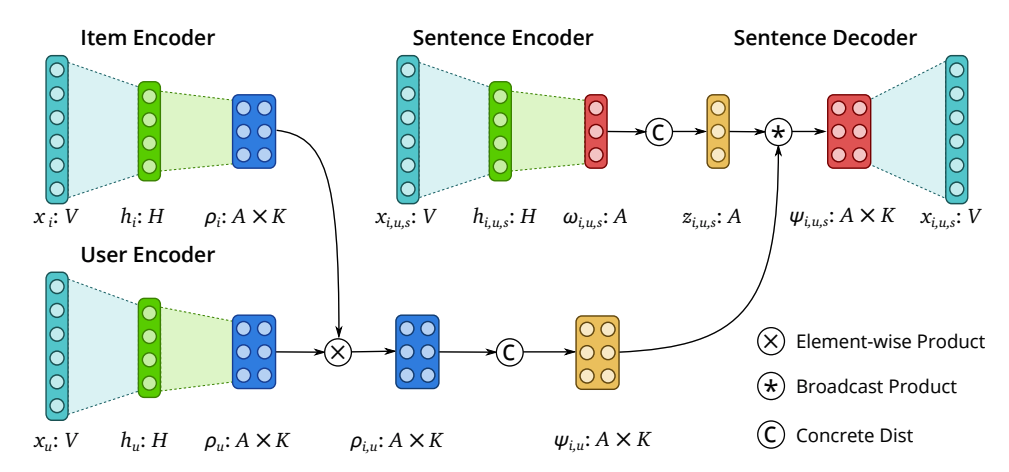
\includegraphics[width=0.9\textwidth]{esmaili-fig1.png}
  \caption{Figure 1 from \cite{esmaeili2018structured}, depicting the structure of VALTA.}
  \label{fig:valta}
\end{figure}

\paragraph{What is the latent structure?}

\paragraph{What is the inference approach?}

\paragraph{If they use amortized inference, what is the amortized model? How many parameters does it have?}

\paragraph{What is the training objective?}

\paragraph{What training / inference approximations does the paper make?}

\paragraph{Does the paper evaluate interpretability? If so how?}

\section{3}

\paragraph{What is the model? Roughly how many parameters does the model have?}

\paragraph{What is the latent structure?}

\paragraph{What is the inference approach?}

\paragraph{If they use amortized inference, what is the amortized model? How many parameters does it have?}

\paragraph{What is the training objective?}

\paragraph{What training / inference approximations does the paper make?}

\paragraph{Does the paper evaluate interpretability? If so how?}

\section{Discussion}

\section{Conclusion}

\bibliographystyle{apalike}
\bibliography{writeup}

\end{document}
